


%% *=*=*=*=*=*=*=*=*=*=*=*=*=*=*=*=*=*=*=*=*=*=*=*=*=*=*=*%
%                   GLOBAL VARIABLES                      %
%% *=*=*=*=*=*=*=*=*=*=*=*=*=*=*=*=*=*=*=*=*=*=*=*=*=*=*=*%
    %%% ENABLES/DISABLES ANNOTATIONS/MESSAGES:
    \newif\ifdraft
    \drafttrue
    % \draftfalse
    
    %%% ENABLES/DISABLES WACV FINAL\SUBMISSION FORMAT:
    \newif\iffinal
    % \finaltrue
    \finalfalse
    
    %%% TITLE OF THE PAPER:
    \def \paperTitle {(?) Automatic Crack Detection in Nuclear Power Plants with Temporal-Spacial Grouping}
    
    %%% ID OF THE PAPER SUBMISSION:
    \def \submissionID {XXX} % *** Enter the wacv Paper ID here
%% *=*=*=*=*=*=*=*=*=*=*=*=*=*=*=*=*=*=*=*=*=*=*=*=*=*=*=*%    
    
    
    
    
%% *=*=*=*=*=*=*=*=*=*=*=*=*=*=*=*=*=*=*=*=*=*=*=*=*=*=*=*%
%               DOCUMENT CONFIG & PACKAGES                %
%% *=*=*=*=*=*=*=*=*=*=*=*=*=*=*=*=*=*=*=*=*=*=*=*=*=*=*=*%
    \documentclass[10pt,twocolumn,letterpaper]{article}
    
    \usepackage{styles/wacv}
    \usepackage[utf8]{inputenc}
    \usepackage{times}
    \usepackage{epsfig}
    \usepackage{graphicx}
    \usepackage{amsmath}
    \usepackage{amssymb}
    
    \usepackage{natbib}
    \usepackage{graphicx}
    
    \usepackage{epstopdf}
    \usepackage{array}
    \usepackage{multirow}
    \usepackage{rotating}
    \usepackage{color}
    \usepackage{tabulary}
    \usepackage{caption} 
    \usepackage[export]{adjustbox}
    \usepackage[pagebackref=true,breaklinks=true,colorlinks,bookmarks=false]{hyperref}
    
    % Use more than one optional parameter in a new commands:
    \usepackage{xargs}                      
    % Todo's package:
    \usepackage[shadow, textwidth=3.1cm, textsize=small]{todonotes}
%% *=*=*=*=*=*=*=*=*=*=*=*=*=*=*=*=*=*=*=*=*=*=*=*=*=*=*=*%




%% *=*=*=*=*=*=*=*=*=*=*=*=*=*=*=*=*=*=*=*=*=*=*=*=*=*=*=*%
%% *=*=*=*=*=*=*=*=*=*=*=*=*=*=*=*=*=*=*=*=*=*=*=*=*=*=*=*%
%                     MACROS START:                       %
%                                                         %
%        These are personal macros and some are           %
%       some are disabled if not a draft version          %
%                                                         %
%% *=*=*=*=*=*=*=*=*=*=*=*=*=*=*=*=*=*=*=*=*=*=*=*=*=*=*=*%
%% *=*=*=*=*=*=*=*=*=*=*=*=*=*=*=*=*=*=*=*=*=*=*=*=*=*=*=*%
    %_______________________________
    %_______________________________
    %% ::VECT SHORTHAND MACRO::
    %-------------------------------
    \newcommand\vect[1]{\boldsymbol{#1}}


    % Macros that are disabled/hidden if not a draft version:
    \ifdraft
        %_______________________________
        %_______________________________
        %% ::COMMENTS MACROs::
        %-------------------------------
        % [Comments on the actual paper's text (Makes the text red)]
        %-------------------------------------------------------------------
            \newcommand\comment[1]{\textcolor{red}{{\tt #1}}}
        
        %_______________________________
        %_______________________________
        % ::MARGIN & INLINE MESSAGES::
        %-------------------------------
        % There are 5 (4 visible) types of messages:
        %   1. "\noteError{...}"    --->  Red Message Bubble
        %   2. "\noteChange{...}"   --->  Purple Message Bubble
        %   3. "\noteInfo{...}"     --->  Light Blue Message Bubble
        %   4. "\noteImprove{...}"  --->  Orange Message Bubble
        %   5. "\noteHidden{...}"   --->  Note that will not show in the PDF
        %-------------------------------------------------------------------
            %% Define message types:
            %%-----------------------
            % NOTE ERROR:
            \newcommandx{\noteError}[2][1=]{\todo[linecolor=red,backgroundcolor=red!25,bordercolor=red,#1]{#2}}
            
            % NOTE CHANGE:
            \newcommandx{\noteChange}[2][1=]{\todo[linecolor=blue,backgroundcolor=blue!25,bordercolor=blue,#1]{#2}}
            
            % NOTE INFO:
            \definecolor{cyann}{rgb}{0,0.8,0.8}
            \newcommandx{\noteInfo}[2][1=]{\todo[linecolor=cyann,backgroundcolor=cyann!25,bordercolor=cyann,#1]{#2}}
            
            % NOTE IMPROVE:
            \definecolor{orange}{rgb}{1,0.5,0}
            \newcommandx{\noteImprove}[2][1=]{\todo[fancyline,linecolor=orange,backgroundcolor=orange!25,bordercolor=orange,#1]{#2}}
            
            % NOTE HIDDEN:
            \newcommandx{\noteHidden}[2][1=]{\todo[disable,#1]{#2}}
            
        \setlength{\marginparwidth}{2.8cm}
        \makeatletter
        \tikzstyle{notestyleraw}=[
          draw=\@todonotes@currentbordercolor,
          fill=\@todonotes@currentbackgroundcolor,
          line width=0.5pt,
          text width=\@todonotes@textwidth-2.8ex-1pt,
          inner sep=1.0ex,
          rounded corners=4pt
        ]
        \makeatother
        % adjust space for notes
        \usepackage{geometry}
            \geometry{left=6.0cm, right = 0.0cm, marginparwidth=2.9cm}    
        
    \else
        % Disable all annotations and display errors for general comments:
        \newcommand\comment[1]{\errmessage{This is not a draft!! Remove all comments!!}}
        \newcommandx{\noteError}[2][1=]{\todo[disable,#1]{#2}}
        \newcommandx{\noteChange}[2][1=]{\todo[disable,#1]{#2}}
        \newcommandx{\noteInfo}[2][1=]{\todo[disable,#1]{#2}}
        \newcommandx{\noteImprove}[2][1=]{\todo[disable,#1]{#2}}
        \newcommandx{\noteHidden}[2][1=]{\todo[disable,#1]{#2}}
    \fi
        
%% *=*=*=*=*=*=*=*=*=*=*=*=*=*=*=*=*=*=*=*=*=*=*=*=*=*=*=*%





%% *=*=*=*=*=*=*=*=*=*=*=*=*=*=*=*=*=*=*=*=*=*=*=*=*=*=*=*%
%% *=*=*=*=*=*=*=*=*=*=*=*=*=*=*=*=*=*=*=*=*=*=*=*=*=*=*=*%
%                     DOCUMENT START:                     %
%                                                         %
%        This is the actual text of the document.         %
%                                                         %
%% *=*=*=*=*=*=*=*=*=*=*=*=*=*=*=*=*=*=*=*=*=*=*=*=*=*=*=*%
%% *=*=*=*=*=*=*=*=*=*=*=*=*=*=*=*=*=*=*=*=*=*=*=*=*=*=*=*%
    \iffinal
        \wacvfinalcopy
    \fi
    
    \def\wacvPaperID{\submissionID} 
    \def\httilde{\mbox{\tt\raisebox{-.5ex}{\symbol{126}}}}
    
    \ifwacvfinal\pagestyle{empty}\fi
    
    \begin{document}
    
        \ifdraft
            % Increase Paper size for margin notes..
            \pdfpageheight 14in 
            \pdfpagewidth 11in
        \fi
    
        \title{\paperTitle}
        
        \author{Authors$^\ast$ \\
            \begin{tabular}{c c} $^\ast$~Univ. of North Carolina at Charlotte\\Charlotte, NC 28223\\\end{tabular}\\
            {\tt \small author@uncc.edu  } 
        }
        
        \maketitle
        
        \begin{abstract}
            \noteError{[Example of comment bubble]: TODO :: Abstract is not present}
[Abstract Here]
        \end{abstract}
        
\section{Introduction}

    %%%%%%%%%%%%%%%%%%%%%%%%%%%%%%%%%%%%%%%%%%%%%%%%%%%%%
    %%%          Comments Examples:
    %%%%%%%%%%%%%%%%%%%%%%%%%%%%%%%%%%%%%%%%%%%%%%%%%%%%%
    % // ---> Inline examples (these affect the layout slightly): 
        %  \noteHidden[inline]{example of inline noteHidden}
        %  \noteInfo[inline]{example of inline noteInfo}
        %  \noteError[inline]{example of inline noteError}
        %  \noteChange[inline]{example of inline noteChange}
        %  \noteImprove[inline]{This needs noteImprove}
    
    
    %% ------------------------------------------------
    %                 Teaser Figure:
    %% ------------------------------------------------
    \begin{figure} [ht]
    
        \begin{centering}
        \begin{tabular}{c}
            \includegraphics[width=0.8\columnwidth]{Images/WeldingCrack2.png} \\
            \includegraphics[width=0.8\columnwidth]{Images/ScratchCrack2.png}
        \end{tabular}
        
        \caption{A few examples of the challenges in detecting cracks in power plants such as: substantial texture due to welding (top), grind and scratch marks (bottom). Though hardly visible due to low contrast and surrounding textures, each of the two images contain only a single crack which we have conveniently centered in the image.}
        \label{challenges}
        \end{centering} 
    \end{figure}
    %% ------------------------------------------------
    
    Structural components of nuclear power plants require periodic inspection to ensure safety requirements and uninterrupted services. The inspection helps agencies to predict future conditions, support investment planning, and allocate limited maintenance and repair resources \cite{Koch:2015}. Typically, certified inspectors or structural engineers manually monitor the videos recorded along the concrete surfaces of the power plant and detect any development of cracks or crack-like defects. Since cracks are rare occurrences, manual inspection is a labor-intensive and tedious process of evaluating 100+ hours of video. Furthermore, since it is costly to close down the power plant for closer investigation, concerns raised by a human inspector about elevated development of cracks needs to be identified and validated for false alarms. Utilization of computer vision for automated crack detection to be used side-by-side with the inspectors is of great interest, not only to reduce false alarm rates and alleviate effort of the inspectors, but also aid in catching more crack related defects onsite. \noteHidden{@Min, would the following sentence describing a crack detection task fit?} Given an input video, the task of an automated crack detection method is to identify a set of frames in that video that contain one or more cracks.
    

  Automatic crack detection poses several challenges, of which a few are depicted in figure \ref{challenges}. First, although the cracks may be modeled as thin edge-like segments, a general model to discriminate a wide range of appearances is very difficult due to lighting and shading conditions at different locations. Second, the images in the recorded video contain highly textured areas including weld and concrete surface which causes fragmented and noisy segmentations. Third, the background from cracks often involves differentiating noise such as scatches and grind patterns which can has similar appearences to cracks. The distinction among scatches, grinds, and cracks becomes even more difficult when an actual crack either overlapped with a scatch or appear inside a grind area.
    

    Summary of recent crack detection methods in the domains of reinforced concrete bridges, precast concrete tunnels, underground concrete pipes, and asphalt pavements can be found in \cite{Koch:2015}.  Most methods follow two steps:
    (1) detection of local features, often using textures; 
    (2) classification of (grouped) features.
    
    Local features have been detected using morphological operations \cite{jahanshahi2013}, Gabor \cite{Medina2014}, 
    \comment{list out what types of texture features} texture features and SVM \cite{chanda2014}, HOG \cite{Kapela2015}, 
    
    
    \comment{List out the features that previous methods have used.  Then briefly mention how many of these are based on a small window.}  The noisy/missing features are filtered/connected using
    segment extending \cite{Liu2008}, tensor voting \cite{Zou2012}, extending a saliency map \cite{Xu2013}, seed growing \cite{Li2011}. 
    
    Then, grouped features have been classified using geometric features with neural network \cite{jahanshahi2013}, 
    
    
    \comment{DON't KNOW WHERE THE REST  FITS in}
    A block SVM classifier with Hough features was used to detect cracks in noisy images HTF-SVM \cite{Hu2010}. 
    
    Unsupervised learning method have also been applied to detect road cracks \cite{Oliveira2014}. 
    
    
    Gabor features along with an Adaboost classifier are used to detect road cracks . Chanda et. al  detect cracks in highly textured bridges using . Kapela et. al. detect asphalt using HOG and a SVM classifier \cite{Kapela2015}. Prasanna et. al. divide the image into blocks, detect lines using RANSAC in each block, extract gradient and intensity features from the block at different scales and then classify the block as crack or not using a classifier \cite{Prasanna2014}. 
    
    
    
    \comment{NOT SURE WHERE THIS FIT IN: and crack saliency \cite{Xu2013}} 
    
    
    
    
    \comment{List them here}.  All methods uses input of single frame thus do not use the spatial-temporal aspects of features.   
    % (I can't think of how to relate Zou) Zou et. has recently used Kalman filter detect defects in weld pipe inspection videos by using a Kalman filter to detect the continuity of the defect motion as compared to just noise detections \cite{Zou2015}. 
    
    
    We propose to improve detection accuracy in two ways.  First, we improve the accuracy of local patches detection by learning features with convolutional neural network.  We collected \comment{XXX} labeled local patches to fine-tune the deep network.  Second, we leverage the expection motion pattern of camera during imaging to group detected local patches in spatio-temporal space, then classify at a group level.  Evaluation using 17 real videos with nearly \comment{170,000 frames of video} demonstrate that spatial-temporal grouping provides \comment{XXX}\% improvement in F-score achieving 86\% true positive rate and 4\% false positive rate.  When compared against two recent methods, our method performed 0.40 higher in F-score on our crack dataset.  
     
     

    % In a survey paper by Koch et. al \cite{Koch:2015} different methods for detecting defects civil infrastructures  were discussed extensively. The authors summarize the different methods of crack detection in the domains of reinforced concrete bridges, precast concrete tunnels, underground concrete pipes, and asphalt pavements. They generalize that all the methods usually have two steps, pre-processing, and crack-identification. The pre-processing involves extracting features from lines or edges. They categorize crack-identification step into 3 categories, threshold-based, model-based, and pattern-based approaches. 

    %% ------------------------------------------------
    %                 Overview Figure:
    %% ------------------------------------------------
    \begin{figure*}
    
        \begin{centering}
        
            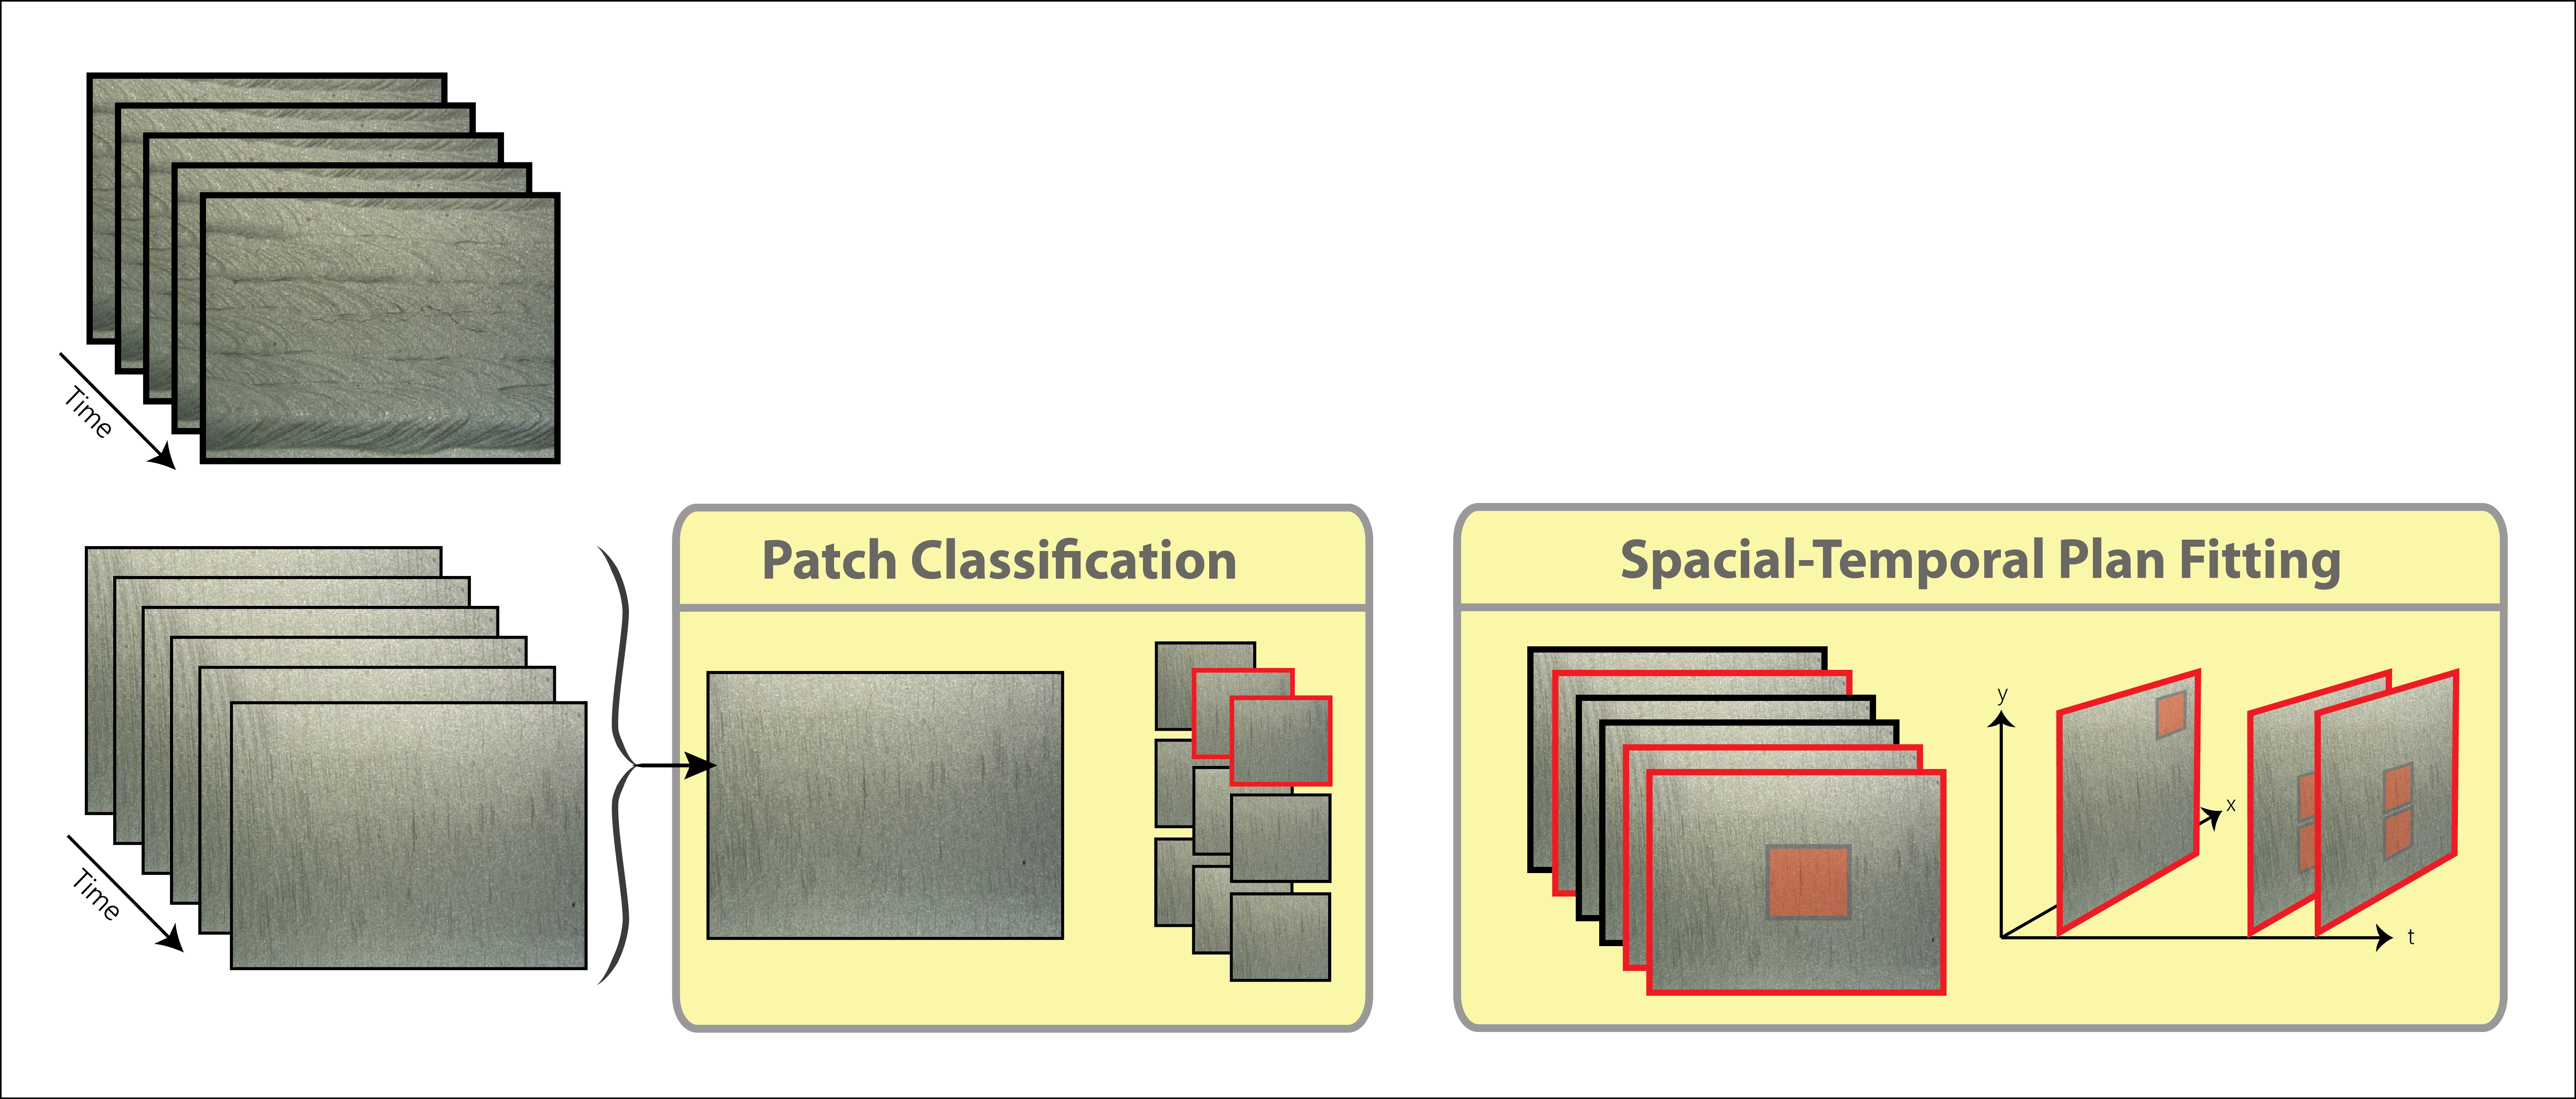
\includegraphics[width=0.6\textwidth]{Images/CrackDiagramDraft.png}
        
            \caption{(Obviously an idea draft) This figure represents the method at an abstract level in a brief glance.}
            \label{fig:FigMain}
            
        \end{centering}
        
    \end{figure*}
    %% ------------------------------------------------

    \paragraph{Related Works}
        Much of the previous research in automatic crack detection has focused on developing a trained classifier using some hand-crafted features. For instance, 
        
        
        
        To reduce false positives, statistical features such as seed growing \cite{Li2011} and crack saliency \cite{Xu2013} have also been applied. 
        
        
        Jahanshahi et al. segment line-like segments using morphological operations, extract geometric features from the segments and then use a neural network classifier to determine if the segment is a crack \cite{jahanshahi2013}. A block SVM classifier with Hough features was used to detect cracks in noisy images HTF-SVM \cite{Hu2010}. Oliveira et. al develop a system to detect road cracks using an unsupervised learning method \cite{Oliveira2014}. Gabor features along with an Adaboost classifier are used to detect road cracks \cite{Medina2014}. Chanda et. al  detect cracks in highly textured bridges using texture features and SVM \cite{chanda2014}. Kapela et. al. detect asphalt using HOG and a SVM classifier \cite{Kapela2015}. Prasanna et. al. divide the image into blocks, detect lines using RANSAC in each block, extract gradient and intensity features from the block at different scales and then classify the block as crack or not using a classifier \cite{Prasanna2014}. Zou et. al detect defects in weld pipe inspection videos by using a Kalman filter to detect the continuity of the defect motion as compared to just noise detections \cite{Zou2015}. 
    
        Instead of hand-crafting the features, Convolutional Neural Networks (CNN) have been utlized to learn features that are useful to the classification task. Use of CNN has met great success in object classification in recent years with the monumental success of Alexnet in the 2012 ImageNet competition \comment{\cite{krizhevsky2012imagenet}}. The GoogLeNet CNN, which is modeled to have less parameters but deeper, performed the best in the 2014 ImageNet Competition \comment{\cite{googlenet2014going}}. Deep Learning CNNs learned in the multi-class object classification can be fine tuned to other tasks such as face detection \comment{\cite{farfade2015multi}} and style classification \comment{\cite{karayev2013styleRecognizing}}. 
        % However, the GoogLeNet framework is too generalized in the context of crack detection \comment{@Steve, can you confirm this?} and its parameters are still in need of fine-tuning to achieve desirable detection performance with a wide range of background pattern and texture.


        Both illumination and contrast vary as a camera is moved across a power plant wall during inspection. If solely classified on individual image patches within the frames then textures such as scratches, welding and grind marks can be frequently and incorrectly considered cracks if the classifier is not strick enough.
        % As previously stated, these false positive detections can be problematic and costly.
        Simply modeling the crack classifier on image patches to be more conservative to reduce false alarms risks reducing its ability to successfully classify actual cracks. 
        Since the inspection for cracks is captured in a sequence of images, we propose to leverage camera motion in video to add spatio-temporal constraint to group and classify detected crack patches. 
        In this paper, we propose to improve the detection of cracks by (1) fine-tuning the GoogLeNet convolutional neural network for crack block classification, and (2) group the detected crack patches by fitting planes in the spatial-temporal space.
        Testing on 17 real videos demonstrates accuracy of \comment{[XX] TP} and \comment{[XX] FP} rates which is \comment{[XX]\%} improvement over prior method. Testing of 42 real images demonstrates 38\% improvement over prior method. %Note that the evaluation of the method is conducted at the classification of image level rather than the segmentation at pixel-level.
        \def \crackPointSet {\vect{D}}
\def \crackPoint {pt}
\def \crackPointi {pt_i}
\def \responseTerm {T}
\def \crackPatchSet {\vect{P_c}}
\def \patch {p}
\def \patchi {p_i}
\def \planTerm {\vect{l}}
\def \planTermi {\vect{l_i}}
\def \threshOneName {span}
\def \threshTwoName {freq}


    %% ------------------------------------------------
    %                 Examples Figure (?):
    %% ------------------------------------------------
    % \renewcommand{\arraystretch}{1.2}
    
    \begin{figure*}
        % \begin{centering}
            
            % 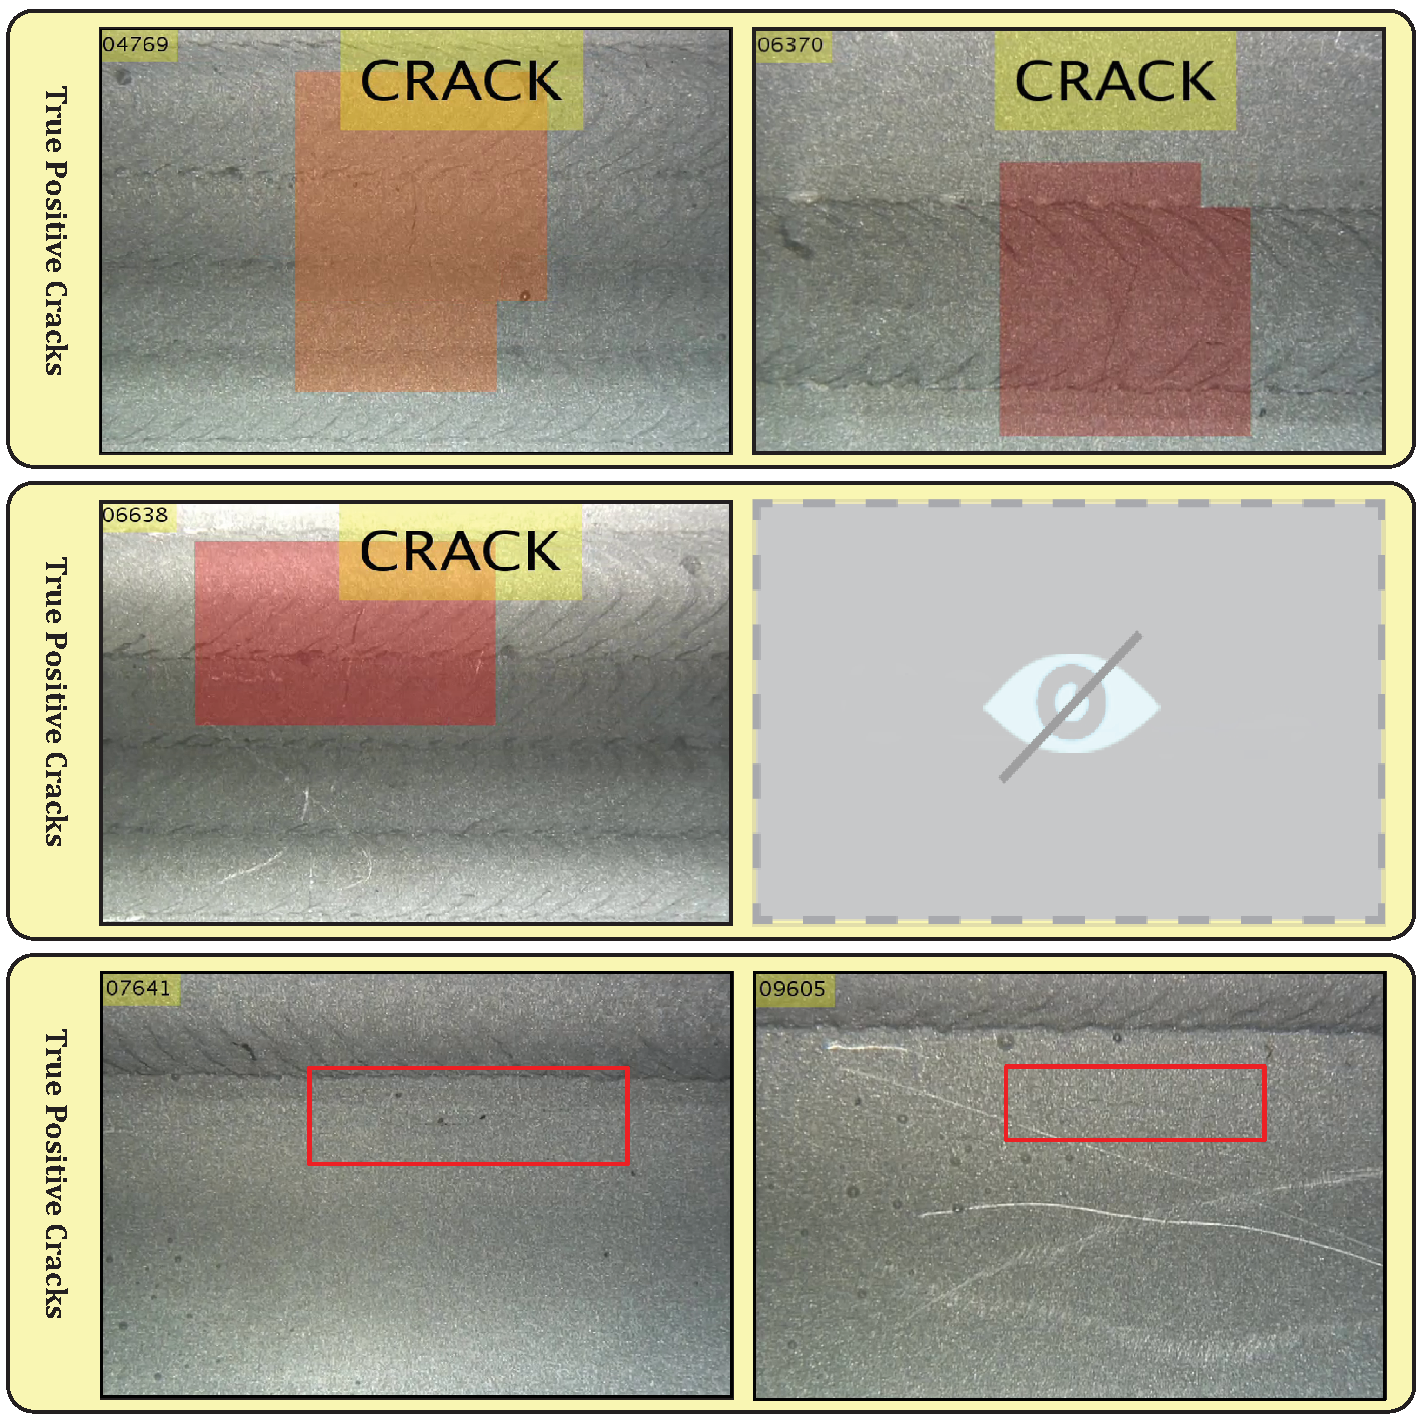
\includegraphics[width=0.92\textwidth,height=0.66\textheight,keepaspectratio]{Images/PerformanceExamples.pdf}
            % 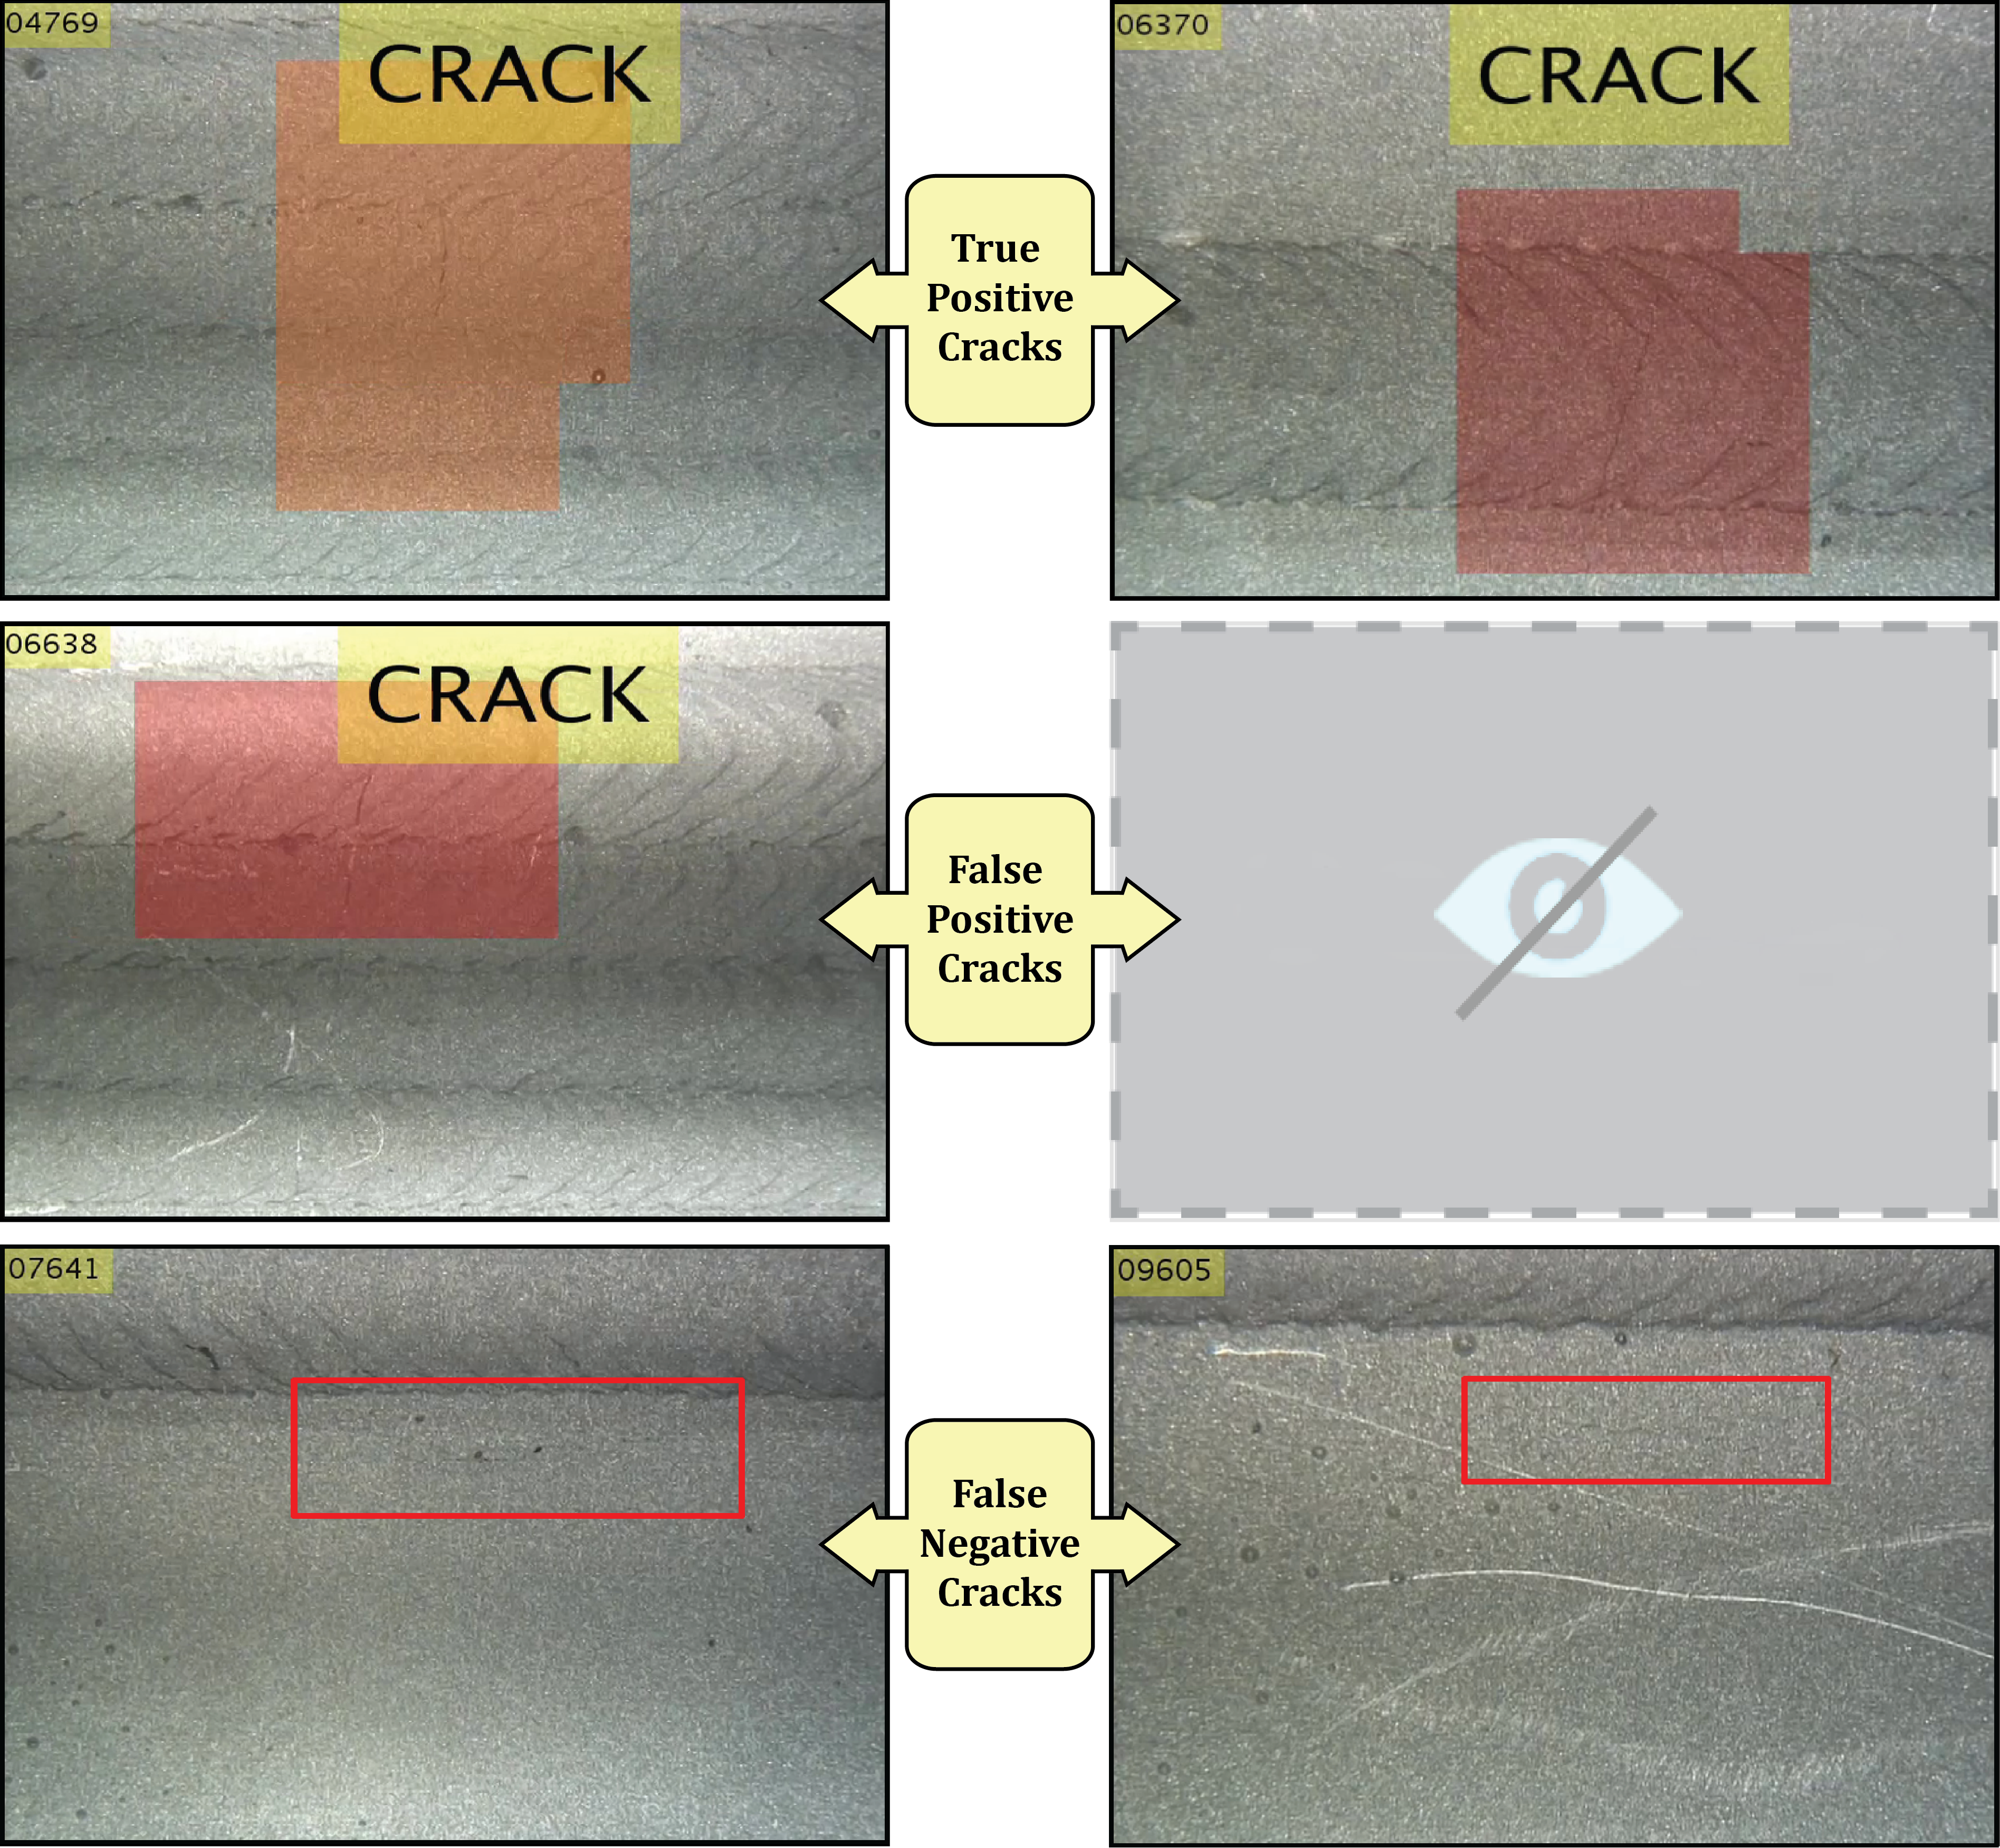
\includegraphics[width=0.92\textwidth,height=0.66\textheight,keepaspectratio]{Images/PerformanceExamples.png}
            \noindent\makebox[\textwidth]{
            \begin{tabular}{cc}
                
                % \centerline{
                    \includegraphics[width=0.43\textwidth,height=0.20\textheight]{Images/TPCrack3.png} &
                    \includegraphics[width=0.43\textwidth,height=0.20\textheight]{Images/TPCrack4.png} \\
                    \multicolumn{2}{c}{(a) True positive cracks detections} \\
                    
                    \includegraphics[width=0.43\textwidth,height=0.20\textheight]{Images/FPCrack3.png} &
                    \includegraphics[width=0.43\textwidth,height=0.20\textheight]{Images/NoVisualHolder.png} \\
                    \multicolumn{2}{c}{(b) False positive cracks detections} \\
                    
                    \includegraphics[width=0.43\textwidth,height=0.20\textheight]{Images/FNCrack3.png} & 
                    \includegraphics[width=0.43\textwidth,height=0.20\textheight]{Images/FNCrack4.png} \\
                    \multicolumn{2}{c}{(c) False negative cracks detections}
                % }
            \end{tabular}
            }
        % \end{centering}
        
        
        \caption{Classification examples of the proposed method. The images in the top each contained a single crack that was correctly identified. The images in the middle row contain no cracks but were falsely identified as crack images. The bottom row shows examples of difficult cracks that were missed.}
        \label{fig:FigExample}
        
    \end{figure*}
    
    %% ------------------------------------------------


\section{Overview}
    % We propose a method to reduce the number of false positives that does not sacrifice, but improves true detection rates on crack containing frames by leveraging spatial and temporal information of the inspection video.
    We refer to fix sized subregions of a video frame $f$ as an image patch $\patch$. For determining whether image patches potentailly contain a crack, a CNN is fine tuned with positive and negative patches taken from a manually labeled dataset \ref{detection}.  During testing, image patches classified as potentially containing cracks are represented as a 3$-$dimensional point cloud and grouped across all frames of the inspection video into special-temporal planes using RANSAC plane fitting \ref{planes}. These planes are then classified as crack containing planes or not through a dual-threshold method with statistically inferred thresholds, which in turn determines the predicted frames and regions in these frames containing cracks.  


    \subsection{Patch-Level Crack Detection} \label{detection}
            Given the set of frames $\vect{F}$ for a video, each frame $f \in \vect{F}$ is divided into 224x224 pixel patches where adjacent patches contain about 75\% overlap in area. This amount of overlap and block size allows for a finer classification grid across the frame image to be utilized in the spatial-temporal grouping described in \ref{planes}. The ImageNet mean RGB value is subtracted from each patch \comment{as in [X]} and then it is run through the fine-tuned CNN described in \ref{training} and classified as $y \in \{0,1\}$, where $y=1$ is a patch that possibly contains a crack.



    \subsection{Spatial-Temporal patch grouping} \label{planes}
            Let $\crackPatchSet$ be the set of patches classified as possibly containing a crack in all frames of the video as described in \ref{detection}. We define a set of potential crack points $\crackPoint \in \crackPointSet$ and perform RANSAC plane fitting and classify the planes to determine cracks at the frame level.

            \paragraph{Plan Fitting}
                Each $\patchi \in \crackPatchSet$ is represented as a 3D point $\crackPointi = (x, y, t)$ where $t$ is the frame number which the patch taken from and $(x,y)$ is the center of the patch. The set $\crackPointSet$ forms a 3D point cloud from where plans are iteratively fit using RANSAC \comment{[X]}. For each plane found, the inlier points of the found plane are removed, and RANSAC plane fitting is run again. This is done until no more planes are found.  For the settings for RANSAC plane fitting, a reference vector of [0, 0, 1] is used. It points approximately parallel to normal vectors of the desired planes with max angle offset between the two vectors of 15 degrees. Each inlier point of the plane has a maximum distance from the surface of the plane of about 500.
            
            \paragraph{Plan Classification} 
                Each plane $\planTerm$ found in during grouping is associated with a set of potential crack points, or $\planTerm = \{\crackPointi\}$ where $\crackPointi \in \crackPointSet$. We classify the planes to determine cracks at the frame level by applying a double threshold on the following features for a given $\planTermi$. Let $\vect{t^{*}}=\{t_i\}$ be the set of distinct time values in the set of crack points $\planTermi$, we can then define:
                \begin{enumerate}
                    \item  $\threshOneName(\planTermi) = \arg\max_{(j,k)}[|\crackPoint_j.t - \crackPoint_k.t|]$ 
                    \item  $\threshTwoName(\planTermi) = \frac{\vect{t^{*}}}{(span(l_i))}$
                \end{enumerate}
                where $\crackPoint_j$ and $\crackPoint_k$ are crack points in $\planTermi$. Frames within the interval of a plan $\planTermi$ are said to contain a crack if:
                
                \begin{gather}
                    \label{DualThresh}
                    \threshOneName(\planTermi) > \lambda_1 $ \text{ } \text{ and } $ \threshTwoName(\planTermi) > \lambda_2
                \end{gather}
                
                 We define the threshold values of $\lambda_1$ and $\lambda_2$ both as the mean minus two standard deviations of patches containing cracks in the training set for $\threshOneName$ and $\threshTwoName$ respectively. 
        
    


   
    
    
    
             



    \subsection{CNN training}
    \label{training}
        We utilize the effectivness of existing CNN classifers, adapted to crack the detection probelm domain, for determining potential cracks on image patches from the video frames. Specifically, a GoogLeNet CNN \comment{\cite{googlenet2014going}} is finetuned by retraining the final inner product layer of the CNN to determine if a image patch has a crack it or not. Approximately 1.5 million 224x224 image patches are extracted from 16 videos for each training set. Crack patches are selected from manually pixel labeled ground truthed crack frames with a crack pixel in the center of the patch. Additional crack patch samples are added by rotating the initial crops by  90 degrees. 
        Classification accuracy and performance during training can be improved by subsampling the non-crack patches based on a morphological response $T$ of the image patches. This is done by first applying to every non-crach patch a morphological operation similar to the approach proposed by Jahanshahi et. al \cite{jahanshahi2013}. $T$ for an image patch $p$ is defined as:
        
        \begin{equation}
                T = \max{[(p \circ \vect{s}) \bullet \vect{s}, p}] - p 
        \end{equation}
        
        where '$\circ$' is the morphological opening operation, '$\bullet$' is the morphological closing and $\vect{s} = S_{[0^o,45^o,90^o,135^o]}$ is the structuring element that defines which neighboring pixels are included in the operation. Weighted sampling, determined by the maximum response $T$ of each of the non-crack patches, is used to select a subsample from the non-crack patches for training. An equal number of positive and negative samples is used during training. The CNN produces a score for each possible classification class and the patch assigned a label from the highest class score as $y \in \{0,1\}$, where $y=1$ is a patch that possibly contains a crack.  
        
         
        \paragraph{Implementation Details}
             The CNN weights are initialized from the GoogLeNet that is available at the Caffe model zoo. The final inner product layer is the layer that is initialized from scratch. We use caffe \cite{jia2014} to finetune train the GoogLeNet by first subtracting mean RGB color of ImageNet from each of the training patches.  The blob learning rate coefficients of the final inner product layer are 10 times higher than the learning rate coefficients from the layers initialized from GoogLeNet.  The base learning rate. is set to  $0.001$,   gamma to $0.1$, momentum $0.9$, and weight decay $0.0005$.  We use a training batch size of 128 for each iteration for a total of 25,000 iterations.  A softmax classifier is attached to the final layer for classification.
    
    
    
         


        \section{Experimental Evaluation}

    \subsection{Dataset} \label{dataset}
        We have collected 17 videos of both real and synthetically laser machined cracks \comment{(Figure 6.)} The videos are captured by Ahlberg MegaRad L Camera approximately 4-6 inches away from the crack samples moving in a raster scan pattern.  There are 45 unique cracks from all the videos which can differ in length, thickness, and distinguishability and are amoungst various degrees of welding, scratches, and grind marks. Each videos contains approximately 10,000 frames.

    \subsection{Evaluation metric}
        All videos have been manually ground truthed at frame level. Frames containing any part of crack(s) are labeled as true.  As videos have been captured in raster scan, each crack would appear to enter and then exit the video.  The exact time point (frame number) of entry/exit is difficult to determine as only a small part of the crack is visible.  So we ignore  25\% of beginning and ending of the ground truthed entry and exit.
        %For use cross-validation for evaluating method performance by using 16 videos for training for the CNN and plane classification and test on the video left out. We a use frame$-$level classification metric. For each video, frames are marked as crack if any part of a crack appears in the frame. In each crack group described in \ref{planes}, the first 25\% of the frames of the crack group and the last 25\% of the crack group are not used in the frame based evaluation and are labeled as “don’t care”. At these times only a small part of the crack is visible, and the crack usually can not be clearly distinguished.
        For each video, the true positive rate (TPR), the false positive rate (FPR) and the F1-score are computed where TP, FP, TN, FN are deteremined at frame-level.
        
        %  \begin{itemize}
        %    \item  $TPR = TP / (TP + FN)$
        %    \item  $FPR = FP / (FP + TN)$
        %    \item  $F1 = (2 * TP) / (2 * TP + FP + FN)$
        %\end{itemize}
        
        %A crack classified frame is TP if any patch in the frame is detected as crack and the ground truth is labeled crack, or FP otherwise. A non$-$crack classified frame is TN if no patches in the frame are detected as crack and the ground truth is labeled non-crack, or FN otherwise. We use True Positive Rate (TPR), False Positive Rate (FPR), and F1-Score to evaluate performance at the frame level. If TP, FP, TN, and FN represent the total number of frames classified as such, then: 
      
    
        \begin{table}
        
            \begin{center}
            
                \begin{tabular}{ l c|c|c| }\\
                    \hline
                        \multicolumn{1}{|l||}{\textbf{Method}} & \textbf{TPR} & \textbf{FPR} & \textbf{F1}\\
                    \hline
                        \multicolumn{1}{|p{2cm}||}{Without Spatio-Temporal} & 0.79 & 0.02 & 0.79 \\
                    \hline
                        \multicolumn{1}{|p{2cm}||}{With Spatio-Temporal} & 0.86 & 0.04 & 0.81 \\
                    \hline
                \end{tabular}
                
                \caption{Frame-level evaluation }
                \label{ResultsFrame}
            
            \end{center}
            
        \end{table}
        
        
        %% ------------------------------------------------
        %   Our dataset method Comparison Examples:
        %% ------------------------------------------------
        \begin{figure*}
        
            \begin{centering}
                \begin{tabular}{c|c|c}
                    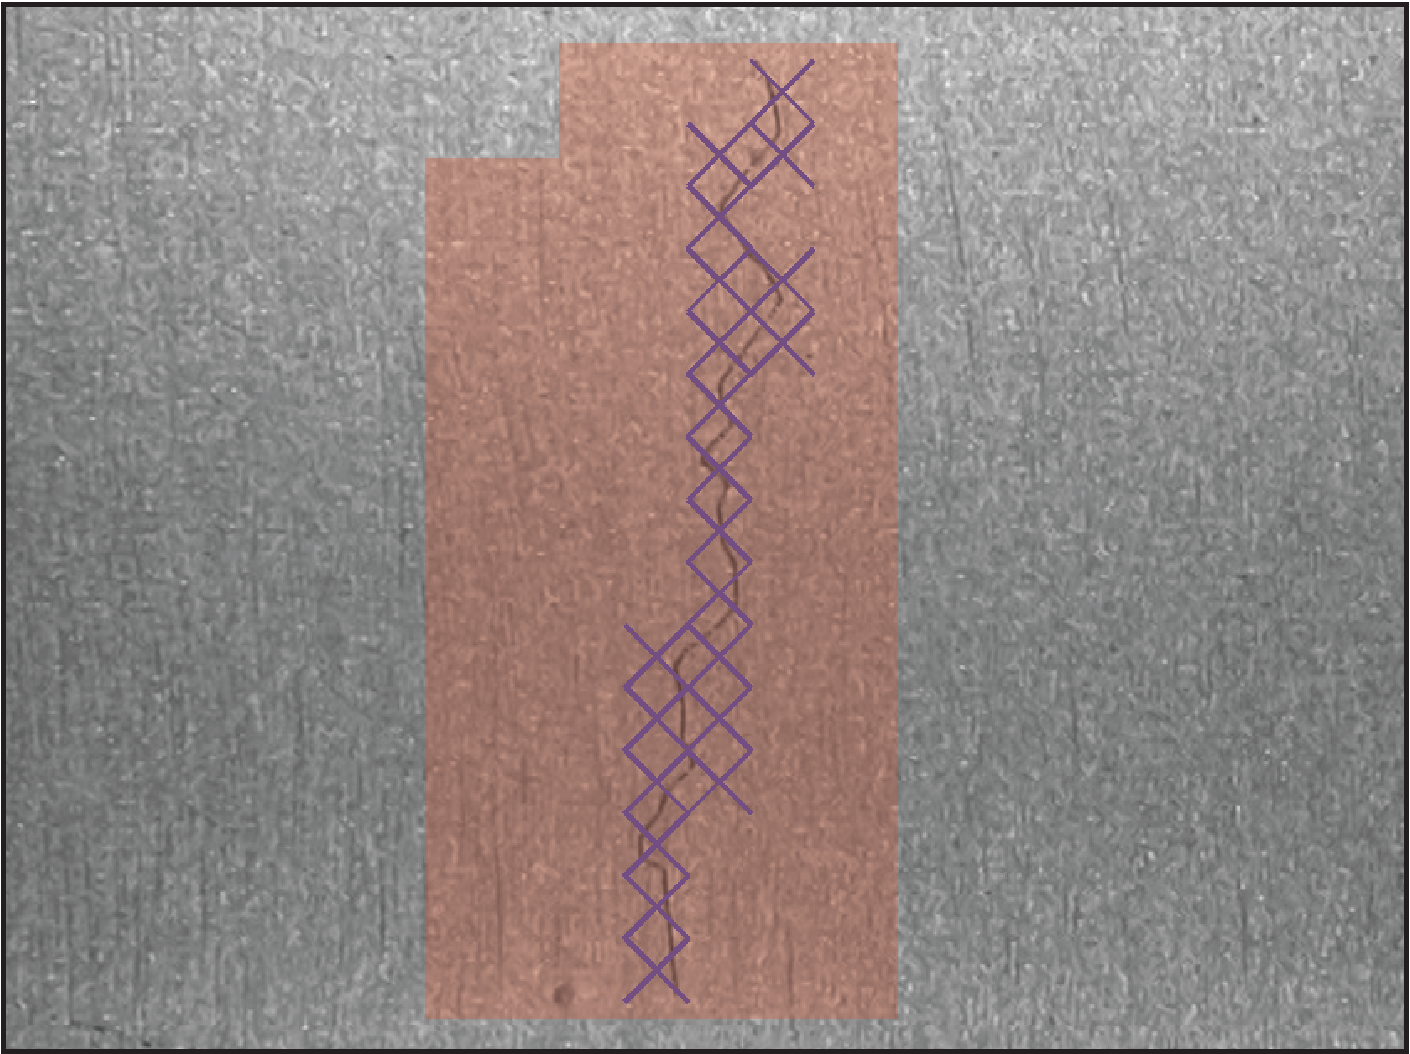
\includegraphics[width=0.3\textwidth]{Images/TP_All_2.pdf} & \includegraphics[width=0.3\textwidth]{Images/TP_us_FN_them_2.png} &
                    \includegraphics[width=0.3\textwidth]{Images/FP_others_2.png} \\
                    (a) TP by all methods & (b) FN by other methods & (c) FP by other method \\
                \end{tabular}
                
                \caption{Our dataset comparison with others. first is all TP, second is TP us and FN them, third is TP us and FP them. I can make them look better later.}
                \label{plantCompareExamples}
                 
            \end{centering}
            
        \end{figure*}
        %% ------------------------------------------------
        
        
        %% ------------------------------------------------
        %   CrackIT dataset method Comparison Examples:
        %% ------------------------------------------------
        \begin{figure*}
        
            \begin{centering}
                \begin{tabular}{c|c}
                    \includegraphics[width=0.45\textwidth]{Images/CrackIT_TP_All-2.png} & \includegraphics[width=0.45\textwidth]{Images/CrackIT_FP_ByCrackIT-2.PNG} \\
                     \\
                    (a) True crack frame detection by all methods & (b) Incorrect crack frame detection by CrackIT
                \end{tabular}
                
                \caption{TODO: figure explaination...}
                \label{crackitExamples}
                 
            \end{centering}
            
        \end{figure*}
        %% ------------------------------------------------
        
        
        %% ------------------------------------------------
        %                 Results Table
        %% ------------------------------------------------
        \begin{table}
        
            \begin{center}
            
                \begin{tabular}{ l c|c|c| }\\
                    \hline
                        \multicolumn{1}{|l||}{\textbf{Method}} & \textbf{TPR} & \textbf{FPR} & \textbf{F1}\\
                    \hline
                        \multicolumn{1}{|p{2cm}||}{CNN} & 0.75 & 0.03 & 0.79 \\
                    \hline
                        \multicolumn{1}{|p{2cm}||}{CrackIT} & 0.79 & 0.60 & 0.33 \\
                    \hline
                        \multicolumn{1}{|p{2cm}||}{Morph} & 0.47 & 0.19 & 0.39 \\
                    \hline
                \end{tabular}
                
                \caption{Results comparison on power plant crack dataset. 346 images (0.25\% of entire frames of dataset) are used to compare performance between algorithms. A frame based evaluation is used. If any blocks in the image are classified as crack, the image is classified as having a crack. CrackIT uses training learned from road crack dataset. The input image resolution size was tuned for the CrackIT algorithm to account for the smaller size image and smaller thickness of nuclear cracks.}  
                \label{ResultsComparisonNuclearDataSet}
            
            \end{center}
            
        \end{table}
        
        \begin{table}
        
            \begin{center}
            
                \begin{tabular}{ l c|c|c| }\\
                    \hline
                        \multicolumn{1}{|l||}{\textbf{Method}} & \textbf{TPR} & \textbf{FPR} & \textbf{F1}\\
                    \hline
                        \multicolumn{1}{|p{2cm}||}{CNN} & 1.00 & 0.00 & 1.0 \\
                    \hline
                        \multicolumn{1}{|p{2cm}||}{CrackIT} & 1.00 & 0.25 & 0.98 \\
                    \hline
                        \multicolumn{1}{|p{2cm}||}{Morph} & 1.00 & 0.00 & 1.00 \\
                    \hline
                \end{tabular}
                
                \caption{Results comparison on CrackIT road crack dataset. 48 images (40 crack images 8 non-crack) are used to compare performance between algorithms. A frame based evaluation is used. If any blocks in the image are classified as crack, the image is classified as having a crack. CNN is trained from nuclear power plant dataset. CNN block size was tuned and found to do best with 171x171 block size. A different block size is necessary for CNN to account for the higher resolution of images and the  greater thickness of road cracks.   }
                \label{ResultsComparisonRoad}
            
            \end{center}
            
        \end{table}
        
        %% ------------------------------------------------
        
        
        % \paragraph{Crack-level}
        %     We also evaluate at the crack camera pass level. We use an overlap strategy based on \\cite{HooverGoldgofpaper}. GT Crack groups are created from frames that are consecutively labeled as cracks. GT non-crack groups are created from consecutive frames labeled as non-cracks.  For each crack detected plane interval and GT Crack Group combination, the number of frames of overlap is computed and then the $overlap-percentage = \min( percent-frame-Overlap-with-GT, percent-frame-Overlap-with-detection)$ is computed.   Each GT Crack group is matched to the crack detection group with the highest overlap-percentage if the $overlap-percentage >= 0.1$. This is then counted as a TP.  Each GT Crack Group can only be matched to one crack detection group. 
        %     FNs are the number GT Crack groups that do not get matched to a crack group detection. 
        %     FPs are the number of crack group detections that do not get matched to a GT Crack group.
        %     TNs are the number GT non-crack groups that get matched to non-crack groups from detection using similar overlap criteria as TPs. 

    \subsection{Accuracy}

        \paragraph{Spatial$-$temporal grouping performance}
            We first evaluate the effectiveness of spacial$-$temporal grouping. Table \ref{ResultsFrame} compares the proposed method with and without spatial$-$temporal grouping. 
            Classification of crack frames using only individual image patches (i.e. without spatial$-$temporal grouping) achieved a TPR just under 80\% and a low FPR of 2\%. The addition of spacial$-$temporal grouping improved the TPR of crack frame classification by 8\% with a negligible increase in FP detections for an overall improvement in F1 measure.   
            \comment{The improvoment is mostly on TPRs, the most of benefits is due to better identification of begining and ending of the crack durations. I'm STILL THINKING} 
            

        \paragraph{Comparison with related works}
            Previous works CrackIT \comment{[X]} and Morph \cite{jahanshahi2013} were compared against on two datasets: 1) the nuclear power plant crack data set described in \ref{dataset}, and 2) the pavement crack data set presented in the CrackIT work. The CrackIT method is publicly availble and trained with data from their pavement crack data set. For the power plant data set the input image resolution size was better tunned for the CrackIT algorithm to account for the smaller image size and thickness of nuclear plant cracks. The Morph method was implemented to follow \cite{jahanshahi2013} as closely as possible. For training the artificial neural network of the Morph method, we used both actual and synthetically generated positive and negative examples of cracks nuclear power plants as the process describes in their work.  Please note that we only compare the results of the proposed method without spacial$-$temporal grouping for a better comparison with the related works and that only 0.25\% of the frames were used for this method comparison. 
            
            Table \ref{ResultsComparisonNuclearDataSet} shows the results of each method for crack frame classification on the nuclear power plant data set. The CrackIT method showed a slight improvement over the proposed method only in terms of TPR, but also had a large performance drop in FPR resulting in the lowest F1 score of the methods compared.  The proposed method displayed the best F1 score by a considerable margin over the other methods.  \comment{We need to add why and link to what's unique about our method.  Since this does not involve grouping, this has to be all about convNN performance.  Our method uses much larger area for computing features and uses (convNN) 224x224 pixel (I think that other two methods uses much smaller window, Steve can check this).  Also, morph method classifies each connected component based on geometric features.  In our dataset, the difference between crack and non-crack in geometry is very subtle}
            
            For pavement crack data set \comment{[X}}, Table \ref{ResultsComparisonRoad} shows the performance of each of the methods for frame crack classification. For the proposed method on the pavement crack data set, image patches of size 171$x$171, which were still resized into 224$x$224 to input to the CNN, were used to account for the smaller image sizes of the data set.  \comment{talk about training of the methods}
            By the perfect performance scores of both the proposed and Morph method, we can tell that the data set is considerably less difficult. This can also we qualitatively confirmed by visual inspection of the data set images, for example \ref{crackitExamples}. 
            
            
        
        
        
        

        
\section{Conclusion and Future Work}
    \noteError{TODO :: Conclusion and future work are not present}
    [Conclusion Here]



        
        \bibliographystyle{styles/ieee}
        \bibliography{section/z-References}
    
    \end{document}
    
    \documentclass{article}
